\documentclass[a4paper,12pt]{article}
\usepackage{amsmath,amsfonts,amsthm}
\usepackage[unicode, final, colorlinks=true]{hyperref}
\usepackage[T1]{fontenc}
\usepackage[utf8]{inputenc}
\usepackage[dvipsnames]{xcolor}
\usepackage{tikz, pgfplots}
\usepackage{tikzscale}
\pgfplotsset{compat=1.17}
\usepgfplotslibrary{groupplots}
\usepgfplotslibrary{fillbetween}
\usetikzlibrary{backgrounds}
\usetikzlibrary{arrows.meta}
\pgfplotsset{plot coordinates/math parser=false}
\usetikzlibrary{external}
\usepgfplotslibrary{patchplots}
\usetikzlibrary{shapes.geometric}
\usetikzlibrary{backgrounds}
\usetikzlibrary{intersections}
\usetikzlibrary{spy}

\newcommand{\ddt}{\partial_t}

\newcommand{\ddx}{\partial_x}

\begin{document}

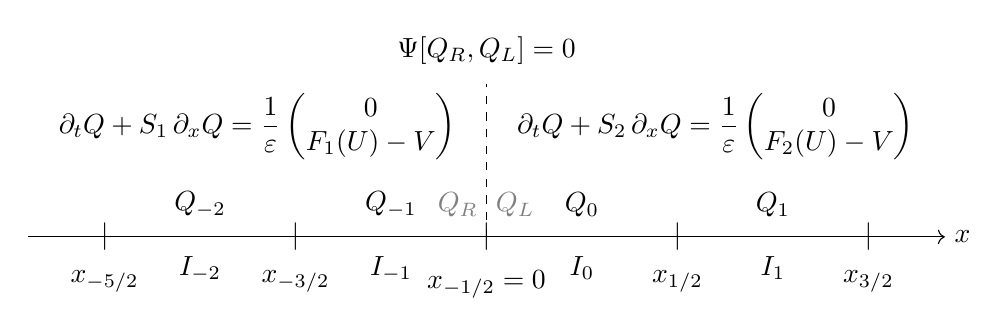
\begin{tikzpicture}[x=\linewidth/25,y=\linewidth/25]%
\draw[->, thin] (-12,0) -- (12,0) node[right] {$x$};
\node[label=below:$x_{-5/2}$] at (-10, 0){$|$};
\node[label=below:$I_{-2}$] at (-7.5, 0){};
\node[label=above:$Q_{-2}$] at (-7.5, 0){};
\node[label=below:$x_{-3/2}$] at (-5, 0){$|$};
\node[label=below:$I_{-1}$] at (-2.5, 0){};
\node[label=above:$Q_{-1}$] at (-2.5, 0){};
\node[label=above:$ \color{gray}Q_{R}$] at (-0.75, 0){};
\node[label=below:{$x_{-1/2}=0$}] at (0, 0){$|$};
\node[label=above:$ \color{gray}Q_{L}$] at (0.75, 0){};
\node[label=below:$I_0$] at (2.5, 0){};
\node[label=above:$Q_0$] at (2.5, 0){};
\node[label=below:$x_{1/2}$] at (5, 0){$|$};
\node[label=below:$I_1$] at (7.5, 0){};
\node[label=above:$Q_1$] at (7.5, 0){};
\node[label=below:$x_{3/2}$] at (10, 0){$|$};
\draw[-, thin, dashed] (0, 0) -- (0, 4) node[label=above:{$\Psi[Q_R, Q_L]=0$}] {};
\coordinate (A) at (-5,1);
\node[label=above:{$\begin{aligned}
  \ddt Q + S_1 \, \ddx Q = \frac{1}{\varepsilon}
                      \begin{pmatrix}
                        0 \\
                        F_1(U) - V
                      \end{pmatrix}
                     \end{aligned}$}] at (-6, 1.5) {};
\node[label=above:{$\begin{aligned}
                      \ddt Q + S_2 \, \ddx Q = \frac{1}{\varepsilon}
                      \begin{pmatrix}
                        0 \\
                        F_2(U) - V
                      \end{pmatrix}
                     \end{aligned}$}] at (6, 1.5) {};
\end{tikzpicture}

\end{document}